%
\documentclass[12pt, a4paper, twoside]{article}


%--Packages--
\usepackage[english]{babel} %if you want index titles and bibliography titles in Swedish comment this line and uncomment the following line
%\usepackage[swedish]{babel}
\usepackage[utf8]{inputenc}
\usepackage[T1]{fontenc}
%\usepackage{showkeys} it show the label you have given to environment equation. Useful when you are writing. Remember to uncomment it before submitting
\usepackage{latexsym,amsmath,amsthm,bm,lmodern,titlesec,xcolor,graphicx,setspace,pdfpages,
geometry,marginnote,caption,array,sectsty,siunitx,eurosym,colortbl,float,wrapfig,vmargin,tikz,hyperref,amssymb,ytableau}
\usepackage[nottoc]{tocbibind}
\usepackage{subfiles}
\usepackage{bbm}
\usetikzlibrary{arrows.meta}

\setpapersize{A4}
\setmarginsrb{30mm}{20mm}{30mm}{30mm}%left top right bottom
                 {8mm}{6mm}{10mm}{10mm}%headheight headsep footheight footskip

% Some useful colors
\definecolor{Rosso}{RGB}{232,61,61}
\definecolor{Viola}{RGB}{188,30,188}
\definecolor{Celeste}{RGB}{34,186,211}
\definecolor{Arancione}{RGB}{232,181,19}
\definecolor{Blu}{RGB}{0, 44, 92}
\definecolor{Azzurro}{RGB}{57,186,238}

\usepackage{booktabs}
  \setlength\heavyrulewidth{0.20ex}
  \setlength\cmidrulewidth{0.10ex}
  \setlength\lightrulewidth{0.10ex}

\hypersetup{colorlinks=true,linkcolor=Blu,allbordercolors=white, urlcolor=blue, citecolor=Viola}
\usepackage{enumitem} 
\renewcommand\labelitemi{\textbullet} 


% math environments
%  we use \newtheorem to specify our theorem-like environments
   % (theorem, definition, etc.) and how to display and number them.
   %
   % Note: The \theoremstyle declarations affect the appearance of the
   % Theorems, Definitions, etc.
   % Note 2: If you want swedish names you have to go and change the argument in brackets e.g. \newtheorem{thm}[defi]{Theorem} should become \newtheorem{thm}[defi]{Sats}
\theoremstyle{definition}
\newtheorem{definition}{Definition}[section]

\theoremstyle{example}
\newtheorem{example}{Example}[section]

\newtheorem*{problem}{Problem}
\newtheorem{conjecture}[definition]{Conjecture}

\theoremstyle{plain}
\newtheorem{theorem}{Theorem}[section]
\newtheorem{proposition}{Proposition}[section]
\newtheorem{corollary}{Corollary}[section]
\newtheorem{lemma}{Lemma}[section]

\theoremstyle{remark}
\newtheorem*{question}{Question}
\newtheorem{remark}[definition]{Remark}
%\newtheorem{example}[definition]{Example}
\newtheorem*{notation}{Notation}


\onehalfspacing


%--Heading of  section--
\titleformat{\section}[display]
  {\normalfont\bfseries\color{Blu}}
  {\filleft
    \begin{tikzpicture}
    \node[
      outer sep=0pt,
      text width=2.5cm,
      minimum height=3cm,
      fill=white,
      font=\color{Blu}\fontsize{80}{0}\selectfont,
      align=center
      ] (num) {\thesection};
    \node[
      rotate=90,
      anchor=south,
      font=\color{black}\large\normalfont
      ] at ([xshift=-5pt]num.west) {\Huge\textsc{}};  
    \end{tikzpicture}%
  }
  {10pt}
  {\titlerule\vskip4pt\Huge\sc\sffamily}

%--Heading of subsection--
\newcommand*\numb[1]{%

\begin{tikzpicture}[baseline=-0.7ex]
\node[
  outer sep=0pt,
      text width=0.6cm,
      minimum height=0.6cm,
      fill=Blu,
      font=\color{white}\fontsize{12}{20}\selectfont,
      align=center
      ] (num) {\thesubsection};
\end{tikzpicture}%
}
\titleformat{\subsection}
  {\normalfont\color{Blu}\large\sc\sffamily}{\numb{\thesubsection}}{0.8em}{}

%--Heading subsubsection--
\newcommand*\stocaz[1]{%

\begin{tikzpicture}[baseline=-0.7ex]
\node[
  outer sep=0pt,
      text width=0.8cm,
      minimum height=0.5cm,
      fill=Blu,
      font=\color{white}\fontsize{10}{20}\selectfont,
      align=center
      ] (num) {\thesubsubsection};
\end{tikzpicture}%
}
\titleformat{\subsubsection}
  {\normalfont\color{Blu}\bfseries\sc\sffamily}{\stocaz{\thesubsubsection}}{0.8em}{}
  


\numberwithin{equation}{section}
\numberwithin{figure}{section}
\begin{document}
\ytableausetup{centertableaux}
% This includes the front page (you need to compile the cover.tex separately and have the .pdf available in the same folder as this .tex file).
\setlength{\voffset}{0cm}
\setlength{\hoffset}{0cm}
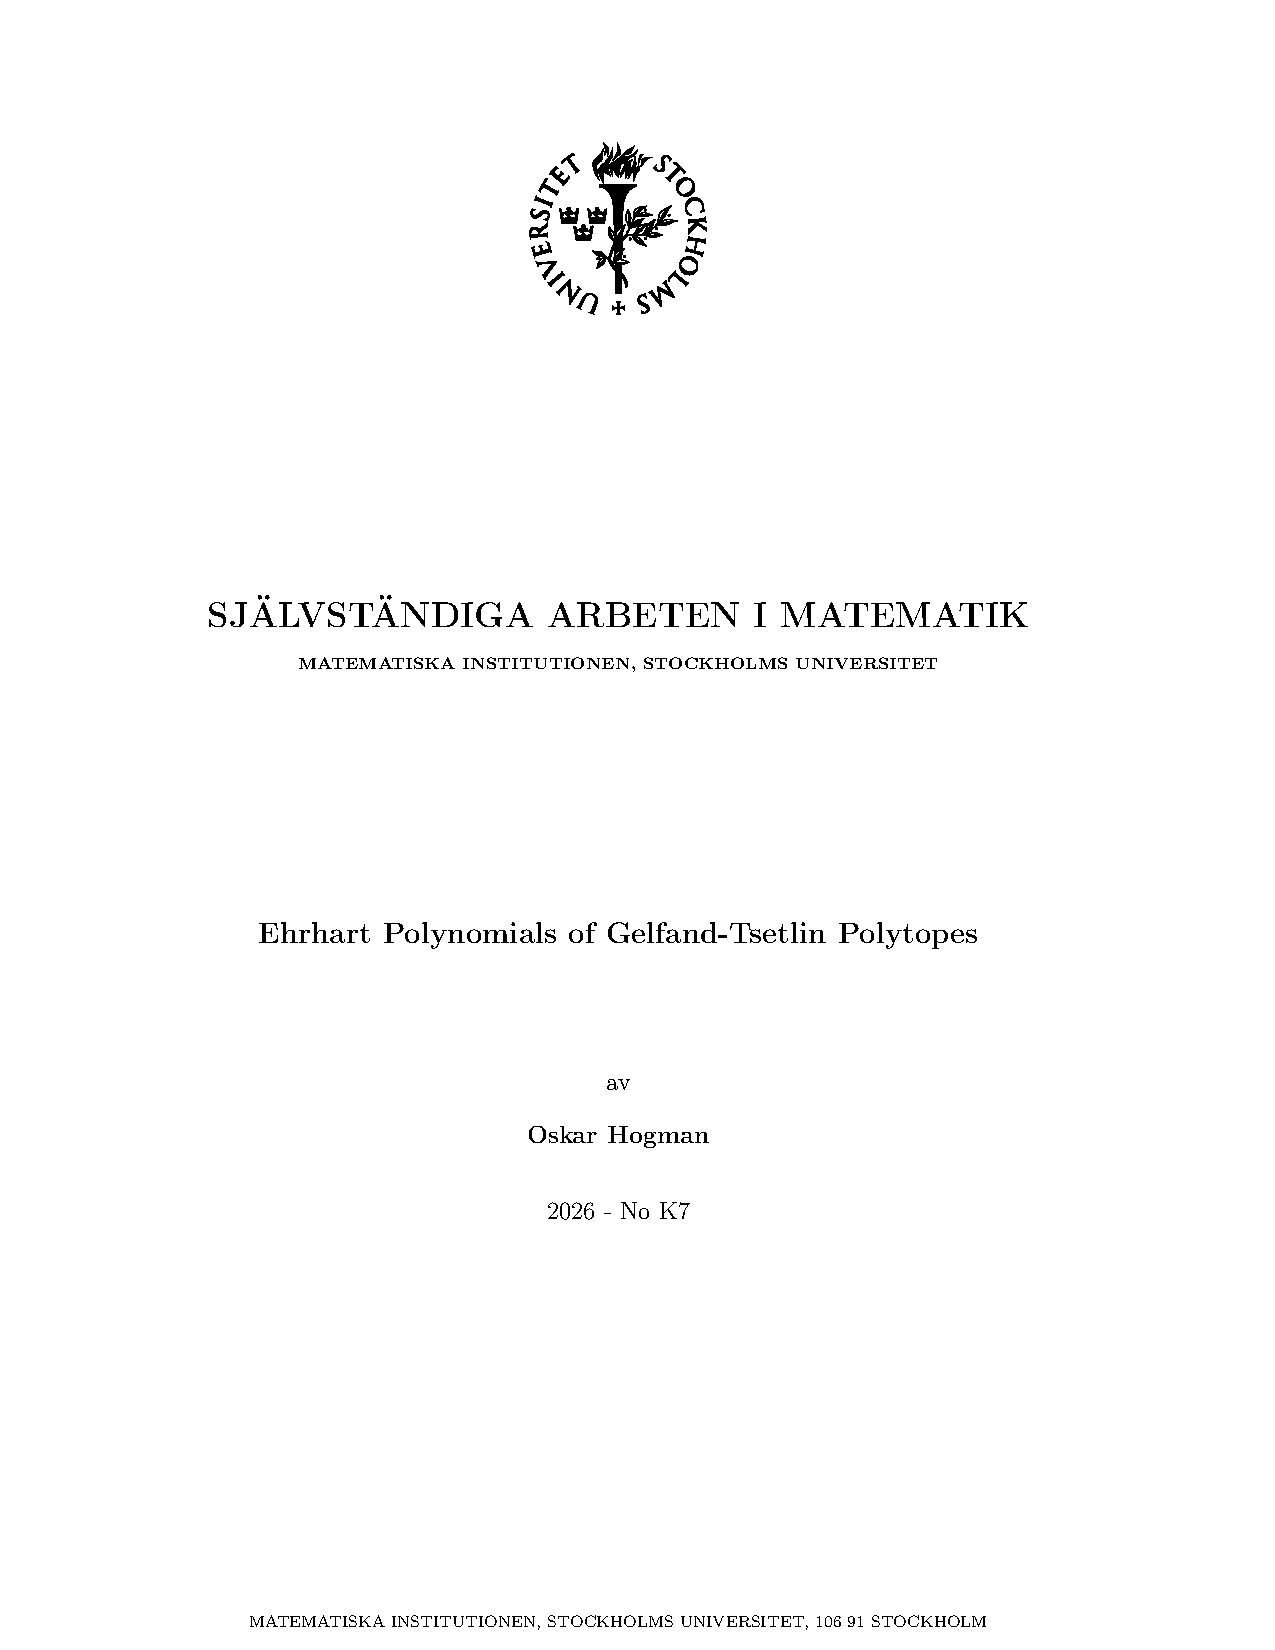
\includepdf[pages={1,2,3,4}]{cover}
\setlength{\voffset}{-2.54cm}
\setlength{\hoffset}{-2.54cm}



\clearpage{\thispagestyle{empty}\cleardoublepage}

\begin{abstract}
    Your summary goes here
\end{abstract}

%create the table of contents
\clearpage{\thispagestyle{empty}\cleardoublepage}
{\hypersetup{linkcolor=black}
\tableofcontents
}
\clearpage

% your first section
%\clearpage{\thispagestyle{empty}\cleardoublepage}
\section{Introduction}
	\subfile{Introduction/Introduction}
\clearpage

%Another section
%\clearpage{\thispagestyle{empty}\cleardoublepage}
\section{Polytopes and Ehrhart theory} \label{polytopes}
	\subfile{Polytopes/Polytopes}
\clearpage

%Another section
%\clearpage{\thispagestyle{empty}\cleardoublepage}
\section{Symmetric functions} \label{symfuncs}
	\subfile{Symmetric-Functions/Symmetric-Functions}
\clearpage

%Another section
%\clearpage{\thispagestyle{empty}\cleardoublepage}
\section{Gelfand-Tsetlin} \label{gt}
	\subfile{GT/GT}
\clearpage

%another section
%\clearpage{\thispagestyle{empty}\cleardoublepage}
\section{Method} \label{method}
	\subfile{Method/Method}
\clearpage

%\clearpage{\thispagestyle{empty}\cleardoublepage}
\section{Results} \label{results}
	\subfile{Results/Results}
%\clearpage


%The section with references.

%\clearpage{\thispagestyle{empty}\cleardoublepage}
\bibliographystyle{alphaurl} %This style prints the urls of online sources.


% All references are to be stored in the file bibliographyFile.bib! 
% It is in the same folder as your main .tex file.
% It is using the bibtex syntax, and you can get these entries from google scholar, etc.
% Your supervisor should know,

\bibliography{bibliographyFile} 

\end{document}
